\section{Preliminary results}

\setcounter{theorem}{0}
\renewcommand{\thetheorem}{A.\arabic{theorem}}
\setcounter{lemma}{0}
\renewcommand{\thelemma}{A.\arabic{lemma}}
\setcounter{proposition}{0}
\renewcommand{\theproposition}{A.\arabic{proposition}}
\setcounter{remark}{0}
\renewcommand{\theremark}{A.\arabic{remark}}

In this section, we prove a key result that rewrites the \gls*{kipld} as a single underdamped Langevin diffusion evolving in $\bR^{d_\theta + N d_x}$ with a rescaled potential function and friction coefficient. This will be useful in the analysis of the \gls*{kipld} and its discretisation, as it allows us to leverage existing results on underdamped Langevin diffusions.
\begin{proposition}\label{prop:kipld_standard_ud}
Let $$(\bm{\theta}_t,\X_t^1,\ldots,\X_t^N,\V_t^\theta,\V_t^{x_1},\ldots,\V_t^{x_N})_{t\geq 0}$$ solve \eqref{eq:KIPLD}. Define
\begin{align*}
\widetilde{\bm{\theta}}_t &:= \bm{\theta}_{\sqrt{N}t}, \qquad
\widetilde{\X}_t^i := N^{-1/2}\X^i_{\sqrt{N}t}, \\
\widetilde{\V}_t^\theta &:= \sqrt{N}\V^\theta_{\sqrt{N}t}, \qquad
\widetilde{\V}_t^{x_i} := \V^{x_i}_{\sqrt{N}t},
\end{align*}
for $i\in[N]$, and set
\begin{align*}
\widetilde{\Z}_t &:= (\widetilde{\bm{\theta}}_t,\widetilde{\X}_t^1,\ldots,\widetilde{\X}_t^N)^\intercal \in \bR^{d_\theta+Nd_x}, \\
\widetilde{\V}_t^z &:= (\widetilde{\V}_t^\theta,\widetilde{\V}_t^{x_1},\ldots,\widetilde{\V}_t^{x_N})^\intercal \in \bR^{d_\theta+Nd_x},
\end{align*}
and
\begin{align}
\bar U_N(\theta,x_1,\ldots,x_N) &:= \frac{1}{N}\sum_{i=1}^N U(\theta,\sqrt{N}\,x_i), \label{eq:barU}
\end{align}
and $\widetilde{\gamma} := \sqrt{N}\gamma$. Then there exists a $\bR^{d_\theta+Nd_x}$-valued Brownian motion $(\widetilde{\B}_t)_{t\ge 0}$ such that
\begin{align}
\md \widetilde{\Z}_t &= \widetilde{\V}_t^z\,\md t, \label{eq:simplesde_scaled} \\
\md \widetilde{\V}_t^z &= -\widetilde{\gamma}\,\widetilde{\V}_t^z\,\md t
- N\nabla_z \bar U_N(\widetilde{\Z}_t)\,\md t
+ \sqrt{2\widetilde{\gamma}}\,\md \widetilde{\B}_t. \nonumber
\end{align}
\end{proposition}
\begin{proof}
By definition of the rescaled variables, we have
\begin{align*}
\md\widetilde{\bm\theta}_t = \md \bm\theta_{s(t)} = \V^\theta_{s(t)}\,\md s(t) = \sqrt{N}\,\V^\theta_{\sqrt N t}\,\md t = \widetilde\V^\theta_t\,\md t
\end{align*}
where $s(t):=\sqrt{N}t$. From \eqref{eq:KIPLD}, $\md \X_t^i=\V_t^{x_i}\md t$, so
\begin{align*}
\md \X^i_{s(t)}
= \V^{x_i}_{s(t)}\md s(t)
= \sqrt{N}\,\V^{x_i}_{\sqrt{N}t}\md t.
\end{align*}
Hence
\begin{align*}
\md \widetilde{\X}_t^i
= N^{-1/2}\,\md \X^i_{\sqrt{N}t}
= N^{-1/2}\,\sqrt{N}\,\V^{x_i}_{\sqrt{N}t}\md t
= \widetilde{\V}_t^{x_i}\md t,
\end{align*}
and therefore $\md \widetilde{\Z}_t=\widetilde{\V}_t^z\md t$. Next, define $\widetilde{\B}_t^j:=N^{-1/4}\B_{\sqrt{N}t}^j$ for $j=0,\ldots,N$; then each $\widetilde{\B}_t^j$ is a Brownian motion and
\(
\md \B_{\sqrt{N}t}^j = N^{1/4}\md \widetilde{\B}_t^j.
\)
Using \eqref{eq:KIPLD}, set $s(t):=\sqrt{N}t$. Then
\small
\begin{align*}
&\md \widetilde{\V}_t^\theta
= \sqrt{N}\,\md \V^\theta_{s(t)}\\
&= \sqrt{N}\left[
\left(-\gamma \V^\theta_{s(t)}
- \frac{1}{N}\!\sum_{i=1}^N \nabla_\theta U(\bm{\theta}_{s(t)},\X^i_{s(t)})\right)\md s(t)
+ \sqrt{\frac{2\gamma}{N}}\,\md \B^0_{s(t)}
\right]\\
&= -N\gamma \V^\theta_{\sqrt{N}t}\md t
- \sum_{i=1}^N \nabla_\theta U(\bm{\theta}_{\sqrt{N}t},\X^i_{\sqrt{N}t})\md t  + \sqrt{2\gamma\sqrt{N}}\,\md \widetilde{\B}_t^0\\
&= -\widetilde{\gamma}\,\widetilde{\V}_t^\theta\md t
- N\nabla_\theta \bar{U}_N(\widetilde{\Z}_t)\md t
+ \sqrt{2\widetilde{\gamma}}\,\md \widetilde{\B}_t^0,
\end{align*}
\normalsize
where we used $\md s(t)=\sqrt{N}\md t$ and
\[
N\nabla_\theta \bar{U}_N(\widetilde{\Z}_t)
= \sum_{i=1}^N \nabla_\theta U(\bm{\theta}_{\sqrt{N}t},\X^i_{\sqrt{N}t}).
\]
Fix $i\in[N]$. Using again $s(t)=\sqrt{N}t$ and \eqref{eq:KIPLD},
\small
\begin{align*}
\md \widetilde{V}_t^{x_i}
&= \md \V^{x_i}_{s(t)}\\
&= \left(-\gamma \V^{x_i}_{s(t)}
- \nabla_x U(\bm{\theta}_{s(t)},\X^i_{s(t)})\right)\md s(t)  + \sqrt{2\gamma}\,\md \B^i_{s(t)} \\
&= -\sqrt{N}\gamma \V^{x_i}_{\sqrt{N}t}\md t
- \sqrt{N}\,\nabla_x U(\bm{\theta}_{\sqrt{N}t},\X^i_{\sqrt{N}t})\md t
 + \sqrt{2\gamma\sqrt{N}}\,\md \widetilde{\B}_t^i\\
&= -\widetilde{\gamma}\,\widetilde{\V}_t^{x_i}\md t
- N\nabla_{z_i}\bar{U}_N(\widetilde{\Z}_t)\md t
+ \sqrt{2\widetilde{\gamma}}\,\md \widetilde{\B}_t^i,
\end{align*}
\normalsize
where
\[
N\nabla_{z_i}\bar{U}_N(\widetilde{\Z}_t)
= \sqrt{N}\,\nabla_x U(\bm{\theta}_{\sqrt{N}t},\X^i_{\sqrt{N}t}).
\]
Stacking coordinates and defining
\(
\widetilde{\B}_t
= (\widetilde{\B}_t^0,\widetilde{\B}_t^1,\ldots,\widetilde{\B}_t^N)^\intercal
\)
gives \eqref{eq:simplesde_scaled}.
\end{proof}

Next we show that the stationary measure of the dynamics in \eqref{eq:simplesde_scaled} is given by a Gibbs measure with potential function $N\bar{U}_N$.
\begin{lemma}[Stationary measure for \eqref{eq:simplesde_scaled}]\label{lem:scaledstat}
The measure $\tilde{\pi}$ invariant for the dynamics in \eqref{eq:simplesde_scaled} is given as
\begin{equation}
\tilde{\pi}(\md \tilde{z}, \md \tilde{v}) \propto \exp\left(-N\bar{U}_N(\tilde{z}) -\frac{1}{2}\|\tilde{v}\|^2\right)\md \tilde{z} \md \tilde{v},
\end{equation}
for all $\tilde{z},\tilde{v}\in\mathbb{R}^{d_z}$, where $d_z=d_\theta+Nd_x$.
\end{lemma}

This result follows directly by observing the rescaling given in Proposition~\ref{prop:kipld_standard_ud} and the standard form of the stationary measure for underdamped Langevin diffusions. We now show that $\bar{U}_N$ is $\mu$-strongly convex under \ref{assump:strongconvexity}.

\begin{lemma}[Strong convexity of $\bar{U}_N$]\label{lem:strongconvexity_barU} Under \ref{assump:strongconvexity}, the function $\bar{U}_N: \bR^{d_\theta + Nd_x} \to \bR$ as defined in \eqref{eq:barU} is $\mu$-strongly convex
\begin{align*}
    \langle z-z^\prime, \nabla \bar{U}_N(z) - \nabla \bar{U}_N(z^\prime)\rangle \geq \mu \|z-z^\prime\|^2,
\end{align*}
for all $z, z^\prime \in \bR^{d_\theta + Nd_x}$ and $N \in \bN$.
\end{lemma}
\begin{proof}
Let
\[
z=(z_\theta,z_1,\dots,z_N),\qquad
z'=(z_\theta',z_1',\dots,z_N').
\]
From
\[
\bar U_N(z)=\frac1N\sum_{i=1}^N U(z_\theta,\sqrt N\,z_i),
\]
we have
\begin{align*}
\nabla_{z_\theta}\bar U_N(z) &=\frac1N\sum_{i=1}^N \nabla_\theta U(z_\theta,\sqrt N z_i), &
\nabla_{z_i}\bar U_N(z) = \frac1{\sqrt N}\nabla_x U(z_\theta,\sqrt N z_i).
\end{align*}
Hence
\begin{align*}
\langle& z-z', \nabla \bar U_N(z)-\nabla \bar U_N(z')\rangle =\frac1N\sum_{i=1}^N
\langle z_\theta-z_\theta',\Delta_{\theta,i}\rangle
+\frac1{\sqrt N}\sum_{i=1}^N
\langle z_i-z_i',\Delta_{x,i}\rangle,
\end{align*}
where
\[
\Delta_{\theta,i}:=\nabla_\theta U(z_\theta,\sqrt N z_i)-\nabla_\theta U(z_\theta',\sqrt N z_i'),
\]
\[
\Delta_{x,i}:=\nabla_x U(z_\theta,\sqrt N z_i)-\nabla_x U(z_\theta',\sqrt N z_i').
\]
Now apply Assumption~\ref{assump:strongconvexity} to the two points
\[
(z_\theta,\sqrt N z_i),\qquad (z_\theta',\sqrt N z_i').
\]
For each \(i\),
\begin{align*}
\langle z_\theta-z_\theta',\Delta_{\theta,i}\rangle
&+\sqrt N\,\langle z_i-z_i',\Delta_{x,i}\rangle
\ge \mu\big(\|z_\theta-z_\theta'\|^2+N\|z_i-z_i'\|^2\big).
\end{align*}
Divide by \(N\) and sum over \(i\):
\begin{align*}
\langle z-z', &\nabla \bar U_N(z)- \nabla \bar U_N(z')\rangle \ge
\mu\|z_\theta-z_\theta'\|^2+\mu\sum_{i=1}^N\|z_i-z_i'\|^2
=\mu\|z-z'\|^2.
\end{align*}
So \(\bar U_N\) is \(\mu\)-strongly convex.
\end{proof}

Next, we show that the function $\bar{U}_N$ is $L$-gradient Lipschitz.
\begin{lemma}[Gradient Lipschitzness of $\bar{U}_N$]\label{lem:gradientlipschitz_barU}
Under \ref{assump:lipschitz}, the function $\bar{U}_N: \bR^{d_\theta + Nd_x} \to \bR$ as defined in \eqref{eq:barU} is $L$-gradient Lipschitz
\begin{align*}
    \|\nabla \bar{U}_N(z) - \nabla \bar{U}_N(z^\prime)\| \leq L \|z-z^\prime\|,
\end{align*}
for all $z, z^\prime \in \bR^{d_\theta + Nd_x}$ and $N \in \bN$.
\end{lemma}
\begin{proof}
Let $z = (z_\theta, z_1, \ldots, z_N)$ and $z^\prime = (z_\theta^\prime, z_1^\prime, \ldots, z_N^\prime)$. Then
\begin{align*}
\|\nabla \bar{U}_N(z) - \nabla \bar{U}_N(z^\prime)\|^2 = & \left\| \frac{1}{N} \sum_{i=1}^N  \left(\nabla_\theta U(z_\theta, \sqrt{N}z_i) - \nabla_\theta U(z_\theta^\prime, \sqrt{N}z_i^\prime)\right)\right\|^2 \\
&+ \frac{1}{N} \sum_{i=1}^N \left\|\nabla_x U(z_\theta, \sqrt{N}z_i) - \nabla_x U(z_\theta^\prime, \sqrt{N}z_i^\prime)\right\|^2.
\end{align*}
Using the fact that $\|\cdot\|^2$ is a convex function and Jensen's inequality for the first term, we obtain
\begin{align*}
\|\nabla \bar{U}_N(z) - \nabla \bar{U}_N(z^\prime)\|^2 &\leq\frac{1}{N} \sum_{i=1}^N \left\|\nabla_\theta U(z_\theta, \sqrt{N}z_i) - \nabla_\theta U(z_\theta^\prime, \sqrt{N}z_i^\prime)\right\|^2\\
& + \frac{1}{N} \sum_{i=1}^N \left\|\nabla_x U(z_\theta, \sqrt{N}z_i) - \nabla_x U(z_\theta^\prime, \sqrt{N}z_i^\prime)\right\|^2.
\end{align*}
Using \ref{assump:lipschitz}, we have
\begin{align*}
\|\nabla \bar{U}_N(z) - \nabla \bar{U}_N(z^\prime)\|^2 &\leq\frac{L^2}{N} \sum_{i=1}^N \left(\|z_\theta - z_\theta^\prime\|^2 + N \|z_i - z_i^\prime\|^2\right)\\
&= L^2 \|z - z^\prime\|^2,
\end{align*}
which completes the proof.
\end{proof}


\setcounter{theorem}{0}
\renewcommand{\thetheorem}{B.\arabic{theorem}}
\setcounter{lemma}{0}
\renewcommand{\thelemma}{B.\arabic{lemma}}
\setcounter{proposition}{0}
\renewcommand{\theproposition}{B.\arabic{proposition}}
\setcounter{remark}{0}
\renewcommand{\theremark}{B.\arabic{remark}}

\section{Equivalence of algorithms}\label{app:algderiv}
We prove in Proposition~\ref{prop:kipld_standard_ud} that the \gls*{kipld} can be rewritten as a single underdamped Langevin diffusion evolving in $\bR^{d_\theta + N d_x}$. This brings the natural question about the algorithms we derived, namely, \gls*{kiplmc1} and \gls*{kiplmc2}, which are discretisations of the KIPLD, and how they relate to the standard discretisation schemes the rescaled diffusion in \eqref{eq:simplesde_scaled}. We show below that the standard discretisations of \eqref{eq:simplesde_scaled} are precisely the \gls*{kiplmc1} and \gls*{kiplmc2} algorithms we defined in Section~\ref{sec:algorithms}. This will later allow us to leverage existing results on the convergence of these standard discretisation schemes to obtain convergence results for our algorithms.

\glsunset{klmc1}

\subsection{KIPLMC1}\label{app:algderivKIPLMC1}
We show below the exponential integrator algorithm, presented in \citep{dalalyan2018sampling}, for our diffusion \eqref{eq:KIPLD} matches the \gls*{kiplmc1} algorithm we defined in Section~\ref{sec:algorithms}.

\begin{proposition}\label{prop:kipld_kiplmc1}
Let the sequence $(\widetilde{Z}_k,\widetilde{V}_k^z)_{k\geq 0}$ be the exponential-integrator discretisation of the rescaled underdamped diffusion \eqref{eq:simplesde_scaled} with friction parameter $\widetilde{\gamma}=\sqrt{N}\gamma$ and step-size $\widetilde{\eta}=\eta/\sqrt{N}$. Define the unscaled variables by
\begin{align*}
\widetilde{\theta}_k &= \theta_k,\qquad \widetilde{X}_k^i = N^{-1/2}X_k^i,\\
\widetilde{V}_k^\theta &= \sqrt{N}V_k^\theta,\qquad \widetilde{V}_k^{x_i} = V_k^{x_i},
\end{align*}
for each $i\in[N]$. Then, after the corresponding rescaling of the Gaussian noise variables, the resulting recursion in $(\theta_k,X_k^i,V_k^\theta,V_k^{x_i})_{i\in[N]}$ coincides exactly with the \gls*{kiplmc1} scheme defined in Section~\ref{subsec:kiplmc1}.
\end{proposition}
\begin{proof}
 Let us recall that, by Proposition~\ref{prop:kipld_standard_ud}, we can rewrite \eqref{eq:KIPLD} as the standard underdamped \gls*{sde}
\begin{align*}
\md \widetilde{\Z}_t &= \widetilde{\V}_t^z\,\md t, \\
\md \widetilde{\V}_t^z &= -\widetilde{\gamma}\,\widetilde{\V}_t^z\,\md t
- N\nabla_z \bar U_N(\widetilde{\Z}_t)\,\md t
+ \sqrt{2\widetilde{\gamma}}\,\md \widetilde{\B}_t,
\end{align*}
where $\tilde{\gamma} = \sqrt{N} \gamma$ is the friction parameter and we also implicitly adjust its initial conditioned to be rescaled. We discretise this diffusion using the exponential integrator scheme (termed \gls*{klmc1}) developed by \citep{dalalyan2018sampling}. In order to do this, define a sequence of functions $\tilde{\psi}_{k+1}^t = \int_0^t \tilde{\psi}_k^s \md s$ where $\tilde{\psi}_0^t = e^{-\tilde{\gamma} t}$. With this definition, the exponential integrator scheme with step-size $\tilde{\eta}$ is defined as
\begin{align*}
\widetilde{Z}_{k+1} &= \widetilde{Z}_k + \tilde{\psi}_1^{\tilde{\eta}} \tilde{V}_k - \tilde{\psi}_2^{\tilde{\eta}} N\nabla_z \bar{U}_N(\widetilde{Z}_k) + \sqrt{2\tilde{\gamma}}\zeta_{k+1}^\prime\\
\widetilde{V}_{k+1} &= \tilde{\psi}_0^{\tilde{\eta}} \widetilde{V}_k - \tilde{\psi}_1^{\tilde{\eta}} N \nabla_z \bar{U}_N(\tilde{Z}_k) + \sqrt{2\tilde{\gamma}} \zeta_{k+1},
\end{align*}
where the stacked vector $[(\zeta_k)_1, \dots, (\zeta_k)_{d_z},(\zeta'_k)_1, \dots (\zeta'_k)_{d_z}]^\top$ is a centred Gaussian random variable with covariance $\widetilde{C}\otimes I_{d_z}$, where $\widetilde{C}$ is given by
\begin{align*}
\widetilde{C} = \int_0^{\tilde{\eta}} \begin{bmatrix} \tilde{\psi}_0^t \\ \tilde{\psi}_1^t \end{bmatrix} \begin{bmatrix} \tilde{\psi}_0^t & \tilde{\psi}_1^t \end{bmatrix} \mathrm{d}t.
\end{align*}
Written explicitly via the definition of $\tilde{\psi}_i^t$, we have,
\small
\begin{equation*}
\widetilde{C}= \frac{1}{2\tilde{\gamma}} \begin{pmatrix}
    (1-e^{-2\tilde{\gamma}\tilde{\eta}}) &  \frac{(e^{-\tilde{\gamma}\tilde{\eta}} -1)^2}{\tilde{\gamma}} \\
    \frac{(e^{-\tilde{\gamma}\tilde{\eta}} -1)^2}{\tilde{\gamma}} &  \frac{2\tilde{\gamma}\tilde{\eta} + 4 e^{-\tilde{\gamma}\tilde{\eta}}- e^{-2\tilde{\gamma}\tilde{\eta}} -3}{\tilde{\gamma}^2}
\end{pmatrix}
\end{equation*}
\normalsize
Let us now relate the matrix $\widetilde{C}$ to the matrix we have defined in \eqref{eq:covariancemat} for the \gls*{kiplmc1} scheme. Written explicitly with the definitions in Section~\ref{subsec:kiplmc1}, \gls*{kiplmc1} instead defines functions $\psi_0^\eta = e^{-\gamma \eta}$ and $\psi_{i+1}^\eta = \int_0^\eta \psi_i^t \md t$, and the covariance matrix in \eqref{eq:covariancemat} is given as
\begin{align*}
C=\frac{1}{2\gamma}
\begin{pmatrix}
    (1-e^{- 2 \gamma\eta}) & \frac{(e^{- \gamma\eta}-1)^2}{\gamma}\\
    \frac{(e^{-\gamma\eta}-1)^2}{\gamma} & \frac{2\gamma\eta + 4e^{-\gamma\eta} - e^{-2\gamma\eta}-3}{\gamma^2}
\end{pmatrix}.
\end{align*}
Recall that the stacked vector $[(\varepsilon_k)_1, (\varepsilon'_k)_1, (\varepsilon_k)_2, (\varepsilon'_k)_2, \dots, ((\varepsilon_k)_{d_z}, (\varepsilon'_k)_{d_z})]^\top$ is a centred Gaussian random variable with covariance $C\otimes I_{d_z}$ as defined in Section~\ref{subsec:kiplmc1}. Note the relation between $\widetilde{C}$ and $C$ is given by
\begin{equation*}
    \widetilde{C}= \begin{pmatrix}
        N^{-\frac{1}{2}} C_{11} & N^{-1} C_{12}\\
        N^{-1} C_{21} & N^{-\frac{3}{2}} C_{22}
    \end{pmatrix}.
\end{equation*}
Hence, we recover
\begin{align*}
\zeta_{k} &= (N)^{-\frac{1}{4}} (\varepsilon_k^0, \dots, \varepsilon_k^N)^\top,\\
\zeta_k^\prime &= (N)^{-\frac{3}{4}} (\varepsilon^{0,\prime}_k, \dots, \varepsilon_k^{N,\prime})^\top.
\end{align*}
We first write the full exponential-integrator scheme coordinatewise, without yet substituting the relations between $\tilde{\eta}$ and $\eta$ or between the rescaled and original variables. This gives
\small
\begin{align*}
\widetilde{\theta}_{k+1} &= \widetilde{\theta}_k + \tilde{\psi}_1^{\tilde{\eta}} \widetilde{V}^\theta_k - \tilde{\psi}_2^{\tilde{\eta}} N \nabla_\theta \bar U_N(\widetilde{Z}_k) + \sqrt{2\tilde{\gamma}}(\zeta_{k}^\prime)^0,\\
\widetilde{X}_{k+1}^i &= \widetilde{X}_k^i + \tilde{\psi}_1^{\tilde{\eta}} \widetilde{V}_k^{x_i} - \tilde{\psi}_2^{\tilde{\eta}} N \nabla_{z_i} \bar U_N(\widetilde{Z}_k) + \sqrt{2\tilde{\gamma}}(\zeta_{k}^\prime)^i,\\
\widetilde{V}_{k+1}^\theta &= \tilde{\psi}_0^{\tilde{\eta}} \widetilde{V}_k^\theta - \tilde{\psi}_1^{\tilde{\eta}} N \nabla_\theta \bar U_N(\widetilde{Z}_k) + \sqrt{2\tilde{\gamma}}(\zeta_{k})^0,\\
\widetilde{V}_{k+1}^{x_i} &= \tilde{\psi}_0^{\tilde{\eta}} \widetilde{V}_k^{x_i} - \tilde{\psi}_1^{\tilde{\eta}} N \nabla_{z_i} \bar U_N(\widetilde{Z}_k) + \sqrt{2\tilde{\gamma}}(\zeta_{k})^i,
\end{align*}
\normalsize
where the noise variables $(\zeta_k)^0$, $(\zeta_k^\prime)^0$, $(\zeta_k)^i$ and $(\zeta_k^\prime)^i$ are the appropriate coordinates of $\zeta_k$ and $\zeta_k^\prime$ respectively. Now recall from Proposition~\ref{prop:kipld_standard_ud} that $\tilde{\gamma} = \sqrt{N}\gamma$, and choose $\tilde{\eta}=\eta/\sqrt{N}$. Then
\begin{align*}
\tilde{\psi}_0^{\tilde{\eta}} &= e^{-\gamma\eta} = \psi_0^\eta,\\
\tilde{\psi}_1^{\tilde{\eta}} &= \frac{1}{\gamma\sqrt{N}} (1-e^{-\gamma\eta}) = \frac{\psi_1^\eta}{\sqrt{N}},\\
\tilde{\psi}_2^{\tilde{\eta}} &= \frac{1}{\gamma N}(\eta - \frac{1}{\gamma}(1-e^{-\gamma\eta})) = \frac{\psi_2^\eta}{N}.
\end{align*}
Using also the identities
\begin{equation}
\begin{aligned}
N\nabla_\theta \bar U_N(\widetilde{Z}_k) &= \sum_{i=1}^N \nabla_\theta U(\widetilde{\theta}_k,\sqrt{N}\widetilde{X}_k^i),\\
N\nabla_{z_i} \bar U_N(\widetilde{Z}_k) &= \sqrt{N}\nabla_x U(\widetilde{\theta}_k,\sqrt{N}\widetilde{X}_k^i),
\end{aligned}\label{eq:grad_rescaling}
\end{equation}
together with $\widetilde{\theta}_k=\theta_k$, $\widetilde{X}_k^i=N^{-1/2}X_k^i$, $\widetilde{V}_k^\theta=\sqrt{N}V_k^\theta$, $\widetilde{V}_k^{x_i}=V_k^{x_i}$, $(\zeta_k)^0=N^{-1/4}\varepsilon_k^0$, $(\zeta_k^\prime)^0=N^{-3/4}\varepsilon_k^{0,\prime}$, $(\zeta_k)^i=N^{-1/4}\varepsilon_k^i$, and $(\zeta_k^\prime)^i=N^{-3/4}\varepsilon_k^{i,\prime}$, we obtain for the $\theta$-coordinates
\small
\begin{align*}
\theta_{k+1} &= \theta_k + \frac{\psi_1^\eta}{\sqrt{N}}\widetilde{V}^\theta_k - \frac{\psi_2^\eta}{N} \sum_{i=1}^N \nabla_\theta U(\theta_k, X_k^i)+ \sqrt{\frac{2\gamma}{N}} \varepsilon^{0,\prime}_{k},\\
\widetilde{V}^\theta_{k+1} &= \psi_0^\eta \widetilde{V}^\theta_k - \frac{\psi_1^\eta}{\sqrt{N}} \sum_{i=1}^N \nabla_\theta U(\theta_k, X_k^i) + \sqrt{2\gamma} \varepsilon^0_{k}.
\end{align*}
\normalsize
Since $\widetilde{V}_k^\theta=\sqrt{N}V_k^\theta$, substituting this relation into the first line and dividing the second line by $\sqrt{N}$ yields
\small
\begin{align*}
\theta_{k+1} &= \theta_k + \psi_1^\eta V^\theta_k - \frac{\psi_2^\eta}{N} \sum_{i=1}^N \nabla_\theta U(\theta_k, X_k^i)+ \sqrt{\frac{2\gamma}{N}} \varepsilon^{0,\prime}_{k},\\
V^\theta_{k+1} &= \psi_0^\eta V^\theta_k - \frac{\psi_1^\eta}{N} \sum_{i=1}^N \nabla_\theta U(\theta_k, X_k^i) + \sqrt{\frac{2\gamma}{N}} \varepsilon^0_{k}.
\end{align*}
\normalsize
For each particle coordinate $i\in[N]$, the same substitutions give
\small
\begin{align*}
\widetilde{X}_{k+1}^i &= \widetilde{X}_k^i + \frac{\psi_1^\eta}{\sqrt{N}}V^{x_i}_k - \frac{\psi_2^\eta}{\sqrt{N}} \nabla_x U(\theta_k, X_k^i)+ \sqrt{\frac{2\gamma}{N}} \varepsilon^{i,\prime}_{k},\\
V^{x_i}_{k+1} &= \psi_0^\eta V^{x_i}_k - \psi_1^\eta \nabla_x U(\theta_k, X_k^i) + \sqrt{2\gamma} \varepsilon^i_{k}.
\end{align*}
\normalsize
Finally, multiplying the first equation by $\sqrt{N}$, i.e. using $X_k^i=\sqrt{N}\widetilde{X}_k^i$, yields
\small
\begin{align*}
X^i_{k+1} &= X^i_k + \psi_1^\eta V^{x_i}_k - \psi_2^\eta \nabla_x U(\theta_k, X_k^i)+ \sqrt{2\gamma} \varepsilon^{i,\prime}_{k}\\
V^{x_i}_{k+1} &= \psi_0^\eta V^{x_i}_k - \psi_1^\eta \nabla_x U(\theta_k, X_k^i) + \sqrt{2\gamma} \varepsilon^i_{k}.
\end{align*}
\normalsize
Together with the $\theta$-update above, this is precisely the \gls*{kiplmc1} scheme.
\end{proof}

\subsection{KIPLMC2}\label{app:algderivKIPLMC2}
\begin{proposition}\label{prop:kipld_kiplmc2}
Let $(\widetilde{Z}_k,\widetilde{V}_k^z)_{k\geq 0}$ be the OBABO discretisation of the rescaled underdamped diffusion \eqref{eq:simplesde_scaled} with friction parameter $\widetilde{\gamma}=\sqrt{N}\gamma$ and step-size $\widetilde{\eta}=\eta/\sqrt{N}$. Define the unscaled variables by
\begin{align*}
\widetilde{\theta}_k &= \theta_k,\qquad \widetilde{X}_k^i = N^{-1/2}X_k^i,\\
\widetilde{V}_k^\theta &= \sqrt{N}V_k^\theta,\qquad \widetilde{V}_k^{x_i} = V_k^{x_i},
\end{align*}
for each $i\in[N]$. Then the resulting recursion in $(\theta_k,X_k^i,V_k^\theta,V_k^{x_i})_{i\in[N]}$ coincides exactly with the \gls*{kiplmc2} scheme defined in Algorithm~\ref{alg:KIPLMC2}.
\end{proposition}
\begin{proof}
In this case we again apply Proposition~\ref{prop:kipld_standard_ud} to apply the OBABO results from \citep{monmarche2021high} for the standard underdamped diffusion, to our own. Let us recall the standard form, given in Proposition~\ref{prop:kipld_standard_ud} with $\tilde{\gamma}=\sqrt{N}\gamma$,
\begin{align*}
\md \widetilde{\Z}_t &= \widetilde{\V}_t^z\,\md t, \\
\md \widetilde{\V}_t^z &= -\widetilde{\gamma}\,\widetilde{\V}_t^z\,\md t
- N\nabla_z \bar U_N(\widetilde{\Z}_t)\,\md t
+ \sqrt{2\widetilde{\gamma}}\,\md \widetilde{\B}_t,
\end{align*}
This diffusion is discretised with the OBABO scheme with step-size $\tilde{\eta}$, to obtain,
\small
\begin{align*}
\widetilde{Z}_{k+1} &= \widetilde{Z}_k + \tilde{\eta} \left(\tilde{\delta}\widetilde{V}_k + \sqrt{1-\tilde{\delta}^2}\xi_{k+1}\right)-\frac{\tilde{\eta}^2}{2} N\nabla_z\bar{U}_N(\widetilde{Z}_k)\\
\widetilde{V}_{k+1}&= \tilde{\delta}^2 \widetilde{V}_{k} + \sqrt{1-\tilde{\delta}^2} (\tilde{\delta}\xi_{k+1} + \xi^\prime_{k+1})-\frac{\tilde{\eta}\tilde{\delta}}{2} N (\nabla_z \bar{U}_N(\widetilde{Z}_k) + \nabla_z \bar{U}_N(\widetilde{Z}_{k+1})),
\end{align*}
\normalsize
where we recall that $\tilde{\delta}=e^{-\tilde{\gamma}\tilde{\eta}/2}$. Let us begin at looking at the discretisation coordinatewise in the scaled case,
\small
\begin{align*}
\widetilde{\theta}_{k+1} &= \widetilde{\theta}_k + \tilde{\eta}\left(\tilde{\delta} \widetilde{V}^\theta_{k} + \sqrt{1-\tilde{\delta}^2} \xi^0_{k+1}\right) - \frac{\tilde{\eta}^2}{2} N \nabla_\theta \bar{U}_N(\widetilde{Z}_k),\\
\widetilde{X}^i_{k+1} &= \widetilde{X}^i_k + \tilde{\eta}\left(\tilde{\delta} \widetilde{V}^{x_i}_{k} + \sqrt{1-\tilde{\delta}^2} \xi^i_{k+1}\right) - \frac{\tilde{\eta}^2}{2} N \nabla_{z_i} \bar{U}_N(\widetilde{Z}_k),\\
\widetilde{V}^\theta_{k+1} &= \tilde{\delta}^2 \widetilde{V}^\theta_k + \sqrt{1-\tilde{\delta}^2} (\tilde{\delta} \xi^0_{k+1} + \xi_{k+1}^{0,\prime}) - \frac{\tilde{\eta}\tilde{\delta}}{2} N(\nabla_\theta \bar{U}_N(\widetilde{Z}_k) + \nabla_\theta \bar{U}_N(\widetilde{Z}_{k+1}),\\
\widetilde{V}^{x_i}_{k+1} &= \tilde{\delta}^2 \widetilde{V}^{x_i}_k + \sqrt{1-\tilde{\delta}^2} (\tilde{\delta} \xi^i_{k+1} + \xi_{k+1}^{i,\prime}) - \frac{\tilde{\eta}\tilde{\delta}}{2} N(\nabla_{z_i} \bar{U}_N(\widetilde{Z}_k) + \nabla_{z_i} \bar{U}_N(\widetilde{Z}_{k+1})).
\end{align*}
\normalsize
We now proceed to rescaling the algorithm by observing that $\tilde{\delta}=\delta$ and recalling that $\tilde{\psi}_0^{\tilde{\eta}} = \psi_0^\eta$. Using this, $\tilde{\eta} = \eta/ \sqrt{N}$ and $\tilde{\gamma} = \sqrt{N}\gamma$ and the identities \eqref{eq:grad_rescaling}, we obtain for the $\theta$-coordinates,
\small
\begin{align*}
\theta_{k+1} &= \theta_k + \frac{\eta}{\sqrt{N}} \left(\delta \widetilde{V}^\theta_k + \sqrt{1-\delta^2}\xi_{k+1}\right) - \frac{\eta^2}{2N}\sum_{i=1}^N\nabla_\theta U(\theta_k, X_k^i)\\
\widetilde{V}^\theta_{k+1} &= \delta^2 \widetilde{V}^\theta_k  + \sqrt{1-\delta^2} (\delta\xi_{k+1} + \xi^\prime_{k+1})
- \frac{\eta\delta}{2\sqrt{N}}\sum_{i=1}^N \bigg(\nabla_\theta U(\theta_k, X_k^i) + \nabla_\theta U(\theta_{k+1}, X_{k+1}^i)\bigg).
\end{align*}
\normalsize
Substituting in the relationship $\widetilde{V}_k^\theta=\sqrt{N}V_k^\theta$ and $\widetilde{X}_k^i = X_k^i/\sqrt{N}$, we obtain,
\small
\begin{align*}
\theta_{k+1} &= \theta_k + \eta \left(\delta V^\theta_k + \sqrt{\frac{1-\delta^2}{N}}\xi_{k+1}\right)
- \frac{\eta^2}{2N}\sum_{i=1}^N\nabla_\theta U(\theta_k, X_k^i)\\
V^\theta_{k+1} &= \delta^2 V^\theta_k  + \sqrt{\frac{1-\delta^2}{N}} (\delta\xi_{k+1} + \xi^\prime_{k+1}) 
- \frac{\eta\delta}{2N}\sum_{i=1}^N \bigg(\nabla_\theta U(\theta_k, X_k^i) + \nabla_\theta U(\theta_{k+1}, X_{k+1}^i)\bigg).
\end{align*}
\normalsize
For the particles $i\in [N]$, the same substitutions give,
\small
\begin{align*}
\widetilde{X}^i_{k+1} &= \widetilde{X}^i_k + \frac{\eta}{\sqrt{N}}\left(\delta V^{x_i}_{k} + \sqrt{1-\delta^2} \xi^i_{k+1}\right) - \frac{\eta^2}{2\sqrt{N}} \nabla_{x_i} U(\theta_k , \sqrt{N}\widetilde{X}_k^i),\\
V^{x_i}_{k+1} &= \delta^2 V^{x_i}_k + \sqrt{1-\delta^2} (\delta \xi^i_{k+1} + \xi_{k+1}^{i,\prime}) - \frac{\eta\delta}{2} (\nabla_{x_i} U(\theta_k, \sqrt{N}\widetilde{X}^i_k)+ \nabla_{x_i} U(\theta_{k+1}, \sqrt{N}\widetilde{X}^i_{k+1})).
\end{align*}
\normalsize
Finally, using $X_k^i = \sqrt{N}\widetilde{X}_k^i$,
we recover,
\small
\begin{align*}
X^i_{k+1} &= X^i_k + \eta \left(\delta V^{x_i}_k + \sqrt{1-\delta^2}\xi^i_{k+1}\right)- \frac{\eta^2}{2}\nabla_x U(\theta_k, X_k^i)\\
V^{x_i}_{k+1} &= \delta^2 V^{x_i}_k  + \sqrt{1-\delta^2} (\delta\xi^i_{k+1} + \xi^{i,\prime}_{k+1}) - \frac{\eta\delta}{2} \bigg(\nabla_x U(\theta_k, X_k^i) + \nabla_x U(\theta_{k+1}, X_{k+1}^i)\bigg).
\end{align*}
\normalsize
This shows that the OBABO discretisation of the rescaled diffusion, with step-size $\tilde{\eta} = \eta/\sqrt{N}$, is precisely the \gls*{kiplmc2} scheme.
\end{proof}
\begin{remark} The results in Propositions~\ref{prop:kipld_standard_ud}--\ref{prop:kipld_kiplmc2} significantly streamline our proofs, since they allow us to connect \gls*{kipld} and our methods \gls*{kiplmc1} and \gls*{kiplmc2} to the standard underdamped diffusion and its discretisations, for which there is a rich literature of results that we can apply.
\end{remark}
\section{Proofs of main results}\label{app:proofs}

\subsection{Proof of Proposition~\ref{prop:stationary}}\label{app:proofstationary}
Given Proposition~\ref{prop:kipld_standard_ud}, the system \eqref{eq:simplesde_scaled} has a stationary measure given by the density
\begin{equation*}
\tilde{\pi}(z, \bar{v}) \propto \exp \left(-N\bar{U}_N(z) - \frac{1}{2}\|\bar{v}\|^2 \right),
\end{equation*}
where $\bar{U}_N$ is given in \eqref{eq:barU}. Let us now look at $\theta$-marginal of this density, which can be written as
\begin{equation*}
\pi_\Theta (\theta) \propto \int
e^{-\sum_{i=1}^N U(\theta, \sqrt{N} z_i) - \frac{1}{2} \|\bar{v}^z\|^2}  \md z_x \md \bar{v}.
\end{equation*}
where $z_x = (z_1, \ldots, z_N) \in \bR^{N d_x}$. Note now that, integrating out $\bar{v}$, using a change of variables $x_i' = \sqrt{N} z_i$, and setting $x' = (x_1', \ldots, x_N')$, we have
\begin{align*}
\pi_\Theta (\theta) &\propto\int_{\mathbb{R}^{Nd_x}} 
e^{-\sum_{i=1}^N U(\theta, x'_i)} \md x', \\
&\propto \left(\int_{\bR^{d_x}} e^{-U(\theta, x') } \md x'\right)^N\\
&= \exp(N \log p_\theta(y)),
\end{align*}
since $p_\theta(y) = \int e^{-U(\theta, x)} \md x$ by definition, where $U(\theta, x) = -\log p_\theta(x, y)$.

\subsection{Proof of Proposition~\ref{prop:mmleerror}}\label{app:proofmmleerror}
Note that, by \ref{assump:strongconvexity}, $U(\theta, x)$ is jointly $\mu$-strongly convex. Let $\kappa(\theta) = - \log p_\theta(y)$. Using the Pr\'{e}kopa-Leindler inequality for strongly log-concave distributions \citep[Theorem~3.8]{saumard2014log}, we can see that
\begin{align*}
\langle \theta - \theta', \nabla \kappa(\theta) - \nabla \kappa(\theta') \rangle \geq \mu \|\theta - \theta'\|^2.
\end{align*}
The bound now follows using Lemma~A.8 from \citep{altschuler2023fasterhighaccuracylogconcavesampling}.

\subsection{Proof of Proposition~\ref{prop:kipld_conv}}\label{app:proofkipld_conv}
By Proposition~\ref{prop:kipld_standard_ud}, the rescaled process
\((\widetilde{\Z}_t,\widetilde{\V}_t^z)\) solves the standard underdamped \gls*{sde}
\begin{equation}\label{eq:proof_kipld_scaled}
\begin{aligned}
\md \widetilde{\Z}_t &= \widetilde{\V}_t^{z}\md t,\\
\md \widetilde{\V}_t^z
&= -\widetilde{\gamma}\widetilde{\V}_t^z\md t
- N \nabla \bar{U}_N(\widetilde{\Z}_t)\md t
+ \sqrt{2\widetilde{\gamma}}\,\md \widetilde{\B}_t,
\end{aligned}
\end{equation}
with $\widetilde{\gamma}=\sqrt{N}\gamma$. By Lemmas~\ref{lem:strongconvexity_barU} and \ref{lem:gradientlipschitz_barU},
\(\bar U_N\) is \(\mu\)-strongly convex and \(L\)-gradient-Lipschitz, hence
\(N\bar{U}_N\) is \(N\mu\)-strongly convex and \(NL\)-gradient-Lipschitz. Define
\[
\widetilde{\mu}:=N\mu,\qquad \widetilde{L}:=NL.
\]
The condition \(\gamma\ge \sqrt{\mu+L}\) implies
\[
\widetilde{\gamma}=\sqrt{N}\gamma \ge \sqrt{N(\mu+L)}=\sqrt{\widetilde{\mu}+\widetilde{L}}.
\]
Therefore Theorem~1 in \citep{dalalyan2018sampling} applies to
\eqref{eq:proof_kipld_scaled} and yields, for \(s\ge 0\),
\begin{align*}
W_2\!\left(\mathcal{L}(\widetilde{\Z}_s),\widetilde\pi_Z\right)
&\le\;
\sqrt{2}\exp\!\left(-\frac{\widetilde{\mu}}{\widetilde{\gamma}}s\right)
W_2\!\left(\mathcal{L}(\widetilde{\Z}_0),\widetilde\pi_Z\right).
\end{align*}
where \(\widetilde\pi_Z\) is the \(\widetilde{\Z}\)-marginal of \(\widetilde{\pi}\)
(Lemma~\ref{lem:scaledstat}).

Now relate rescaled and original time: by definition,
\[
\widetilde{\Z}_{t/\sqrt{N}}
=\big(\bm{\theta}_{t},N^{-1/2}\X_t^1,\ldots,N^{-1/2}\X_t^N\big)^\intercal.
\]
Hence the \(\theta\)-component of \(\widetilde{\Z}_{t/\sqrt{N}}\) is \(\bm{\theta}_t\), and
the \(\theta\)-marginal of \(\widetilde\pi_Z\) is \(\pi_\Theta\). We note
\begin{equation*}
W_2\!\left(\mathcal{L}(\bm{\theta}_t),\pi_\Theta\right)
\le
W_2\!\left(\mathcal{L}(\widetilde{\Z}_{t/\sqrt{N}}),\widetilde\pi_Z\right).
\end{equation*}
Using \(s=t/\sqrt{N}\) gives
\[
\frac{\widetilde{\mu}}{\widetilde{\gamma}}\,\frac{t}{\sqrt{N}}
=\frac{N\mu}{\sqrt{N}\gamma}\,\frac{t}{\sqrt{N}}
=\frac{\mu}{\gamma}t.
\]
Therefore
\begin{equation*}
W_2\!\left(\mathcal{L}(\bm{\theta}_t),\pi_\Theta\right)
\le
\sqrt{2}\exp\!\left(-\frac{\mu}{\gamma}t\right)
W_2\!\left(\mathcal{L}(\widetilde{\Z}_0),\widetilde\pi_Z\right).
\end{equation*}
Finally, with \(\bar Z_\star\sim \widetilde\pi_Z\),
\[
W_2\!\left(\mathcal{L}(\widetilde{\Z}_0),\widetilde\pi_Z\right)
\le \mathbb{E}\!\left[\|\widetilde{\Z}_0-\bar Z_\star\|^2\right]^{1/2},
\]
which is exactly the stated bound (up to the same notation
\(\widetilde{\Z}_0\equiv \Z_0\) used in the proposition).

\subsection{Proof of Theorem~\ref{thm:KPLMC1}}\label{app:proofnumericalKPLMC1}
By Proposition~\ref{prop:kipld_standard_ud}, we can rewrite KIPLD as the standard underdamped diffusion with stationary measure
\begin{align*}
\widetilde{\pi}(z, v) \propto e^{-N \bar{U}_N(z) - \|v\|^2/2}.
\end{align*}
We will now look at the standard kinetic Langevin Monte Carlo discretisation of the \gls*{sde} and show that this scheme coincides with \gls*{kiplmc1} to utilize the bounds in \citep{dalalyan2018sampling} directly.

Let us write the Exponential Integrator discretisation of this scheme as we do in \ref{app:algderivKIPLMC1},
\small
\begin{equation}\label{eq:underdamped_normal_1}
\begin{aligned}
\widetilde{Z}_{n+1} &= \widetilde{Z}_{n} + \widetilde{\psi}_1^{\tilde{\eta}} \widetilde{V}_n^z - \widetilde{\psi}_2^{\tilde{\eta}} N \nabla \bar{U}_N(\widetilde{Z}_n)+ \sqrt{2 \tilde{\gamma}} \zeta_{n+1}',\\
\widetilde{V}_{n+1}^z &= \widetilde{\psi}_0^{\tilde{\eta}} \widetilde{V}_n^z - \widetilde{\psi}_1^{\tilde{\eta}} N \nabla \bar{U}_N(\widetilde{Z}_n) + \sqrt{2 \tilde{\gamma}} \zeta_{n+1}. \end{aligned}
\end{equation}
\normalsize
Since the function $z \mapsto N \bar{U}_N(z)$ is $N\mu$ strongly convex and $NL$-gradient-Lipschitz, for $\tilde{\gamma} \geq \sqrt{N\mu + N L}$ and $\tilde{\eta} \leq \mu / (4 \tilde{\gamma} L)$, \citep[Theorem~2]{dalalyan2018sampling} directly implies that
\small
\begin{align*}
W_2(\nu_n, \widetilde\pi_Z) &\leq \sqrt{2} \mathbb{E}[\|Z_0-\bar{Z}_\star\|^2]^{1/2} \left( 1 - \frac{0.75 \tilde{\mu} \tilde{\eta}}{\tilde{\gamma}}\right)^n + \frac{\tilde{\eta}\tilde{L}}{\tilde{\mu}}\sqrt{2d_z},
\end{align*}
\normalsize
where $\nu_n:=\mathcal L(\widetilde Z_n)$ denotes the law of the position iterate in \eqref{eq:underdamped_normal_1}, $\widetilde\pi_Z$ denotes the position marginal of the stationary measure in Lemma~\ref{lem:scaledstat}, and $\bar Z_\star\sim\widetilde\pi_Z$. We now recall from \ref{app:algderivKIPLMC1}, that $\tilde{\eta}=\eta/\sqrt{N}$ and $\tilde{\gamma}=\sqrt{N}\gamma$, from which we obtain,
\small
\begin{equation*}
W_2(\nu_n, \widetilde\pi_Z) \leq C_1\left(1-\frac{0.75 \mu\eta}{\gamma}\right)^n + \eta C_2,
\end{equation*}
\normalsize
where,
\small
\begin{align*}
C_1&= \sqrt{2} \bE[\|Z_0-\bar{Z}_\star\|^2]^{1/2}, \qquad \bar{Z}_\star\sim \widetilde\pi_Z\\
C_2&=\sqrt{2}\frac{L}{\mu} \sqrt{\frac{d_z}{N}}.
\end{align*}
\normalsize

The rescaling leaves the $\theta$-coordinate unchanged, so the $\theta$-component of $\widetilde Z_n$ is $\theta_n$. Consequently, $\mathcal L(\theta_n)$ and $\pi_\Theta$ are the $\theta$-marginals of $\nu_n$ and $\widetilde\pi_Z$, respectively. Since the coordinate projection $z\mapsto\theta$ is $1$-Lipschitz, $W_2(\mathcal L(\theta_n),\pi_\Theta)\leq W_2(\nu_n,\widetilde\pi_Z)$. Applying this inequality and the triangle inequality, we obtain
\small
\begin{align*}
\mathbb{E}[\|\theta_n-\bar{\theta}_\star\|^2]^{1/2} &= W_2(\mathcal{L}(\theta_n), \delta_{\bar{\theta}_\star})\\
&\leq W_2(\mathcal{L}(\theta_n), \pi_\Theta) + W_2(\pi_\Theta, \delta_{\bar{\theta}_\star})\\
&\leq C_1 \left(1-\frac{0.75 \mu\eta}{\gamma}\right)^n + \eta C_2 + \sqrt{\frac{C_3}{N}},
\end{align*}
\normalsize
where the last term is bounded by Proposition~\ref{prop:mmleerror} with $C_3=d_\theta/\mu$.

\subsection{Proof of Theorem~\ref{thm:KIPLMC2}}\label{app:proofnumericalKPLMC2}
Again, we consider our rescaled standard underdamped diffusion, given by \eqref{eq:simplesde_scaled} and seek to directly apply the results from \citep{monmarche2021high} for our scheme.

We now write the splitting scheme as in \ref{app:algderivKIPLMC2},
\small
\begin{equation}
\begin{aligned}\label{eq:underdamped_normal_2}
\widetilde{Z}_{n+1} &= \widetilde{Z}_n + \tilde{\eta} (\tilde{\delta} \widetilde{V}^z_n + \sqrt{1-\tilde{\delta}^2} \xi_{n+1})- \frac{\tilde{\eta}^2}{2}N \nabla \bar{U}_N(\widetilde{Z}_n)\\
\widetilde{V}^z_{n+1} &= \tilde{\delta}^2 \widetilde{V}_n^z - \frac{\tilde{\eta}\tilde{\delta}}{2}(N\nabla \bar{U}_N(\widetilde{Z}_n) + N \nabla\bar{U}_N (\widetilde{Z}_{n+1}) ) + \sqrt{1-\tilde{\delta}^2}(\tilde{\delta}\xi_{n+1} + \xi_{n+1}^\prime),
\end{aligned}
\end{equation}
\normalsize
where $\tilde{\delta}=e^{-\tilde{\gamma}\tilde{\eta}/2}$.  Set
\begin{align*}
\widetilde\mu&:=N\mu,
&\widetilde L&:=NL,\\
\widetilde\kappa&:=\frac{\widetilde\mu}{3\widetilde\gamma},
&A_N&:=\sqrt{3}\bigl(\sqrt{NL}\lor(NL)^{-1/2}\bigr).
\end{align*}
By Lemmas~\ref{lem:strongconvexity_barU} and~\ref{lem:gradientlipschitz_barU}, the potential $N\bar U_N$ is $\widetilde\mu$-strongly convex and has $\widetilde L$-Lipschitz gradient.  Moreover,
\begin{align*}
\widetilde\gamma\geq2\sqrt{\widetilde L}
&\quad\Longleftrightarrow\quad \gamma\geq2\sqrt L,\\
\widetilde\eta\leq\frac{\widetilde\mu}{33\widetilde\gamma^3}
&\quad\Longleftrightarrow\quad \eta\leq\frac{\mu}{33\gamma^3},\\
1-\widetilde\eta\widetilde\kappa
&=1-\frac{\eta\mu}{3\gamma}=:q.
\end{align*}
Indeed, $\mu\leq L$ and the stated parameter restrictions give
$0<\eta\mu/(3\gamma)\leq\mu^2/(99\gamma^4)\leq1/1584$, so $q\in(0,1)$.
Let $\widetilde P$ be the transition kernel of \eqref{eq:underdamped_normal_2}, let $\widetilde\pi_{\widetilde\eta}$ be its invariant probability measure on phase space, let $\widetilde\pi$ be the invariant probability measure of the diffusion in Lemma~\ref{lem:scaledstat}, and let $\widetilde\pi_Z$ be the position marginal of $\widetilde\pi$.  Theorem~1 of \citep{monmarche2021high} gives, for all $\rho,\sigma\in\mathcal P_2(\mathbb R^{2d_z})$,
\begin{align}
W_2(\rho\widetilde P^n,\sigma\widetilde P^n)
\leq A_Nq^{n/2}W_2(\rho,\sigma).
\label{eq:kiplmc2_phase_contraction}
\end{align}
Proposition~11 of the same reference, applied with $p=2$, gives
\begin{align}
b_N
&:=W_2(\widetilde\pi_{\widetilde\eta},\widetilde\pi)\nonumber\\
&\leq\widetilde\eta\sqrt{d_z}\,
\frac{2A_N\widetilde K}{\widetilde\kappa}
=\eta\sqrt{d_z}\,\frac{6\gamma\widetilde K}{N\mu}\,A_N
=:B_N,
\label{eq:kiplmc2_invariant_bias}
\end{align}
where
\begin{align*}
\widetilde K
:=\widetilde L\left(1+e^{\widetilde L\widetilde\eta^2}
\left(\frac{\widetilde\eta}{6}
+\frac{\widetilde\eta^2\widetilde L}{24}\right)\right)
\left(1+\frac{\widetilde\eta\widetilde L}{2\sqrt{\widetilde\mu}}\right).
\end{align*}

Substituting $\widetilde L=NL$, $\widetilde\eta=\eta/\sqrt N$, and $\widetilde\mu=N\mu$ into $\widetilde K$ yields the exact identity
\begin{align*}
\widetilde K
&=NL\left(1+e^{L\eta^2}
\left(\frac{\eta}{6\sqrt N}+\frac{\eta^2L}{24}\right)\right)\left(1+\frac{\eta L}{2\sqrt\mu}\right).
\end{align*}
Define
\begin{align*}
K:=L\left(1+e^{L\eta^2}
\left(\frac{\eta}{6}+\frac{\eta^2L}{24}\right)\right)
\left(1+\frac{\eta L}{2\sqrt\mu}\right).
\end{align*}
Since $N\geq1$,
\begin{align*}
\widetilde K&\leq NK,
&A_N\leq\sqrt{3N}\bigl(\sqrt L\lor L^{-1/2}\bigr).
\end{align*}
For conciseness, set $M_L:=\sqrt L\lor L^{-1/2}$ and define
\begin{align*}
G_\eta
&:=\frac{6\gamma K}{\mu}M_L\\
&=\frac{6\gamma L}{\mu}M_L \left(1+\frac{\eta L}{2\sqrt\mu}\right)\left(1+e^{L\eta^2}
\left(\frac{\eta}{6}+\frac{\eta^2L}{24}\right)\right).
\end{align*}
To make the implicit constant in Theorem~\ref{thm:KIPLMC2} uniform in $\eta$, set
\begin{align*}
\eta_0&:=\frac{\mu}{33\gamma^3},\\
G_\star
&:=\frac{6\gamma L}{\mu}M_L\left(1+\frac{\eta_0L}{2\sqrt\mu}\right)\left(1+e^{L\eta_0^2}
\left(\frac{\eta_0}{6}+\frac{\eta_0^2L}{24}\right)\right).
\end{align*}
Every factor in $G_\eta$ is nondecreasing for $\eta\geq0$.  Hence the restriction $0<\eta\leq\eta_0$ gives $G_\eta\leq G_\star$, where $G_\star$ depends only on $\mu$, $L$, and $\gamma$.  Consequently, \eqref{eq:kiplmc2_invariant_bias} gives
\begin{align}
B_N
&\leq\eta\sqrt{d_z}\,\frac{6\gamma K}{\mu}\,
\sqrt{3N}\,M_L
\leq\sqrt3\,G_\star\eta\sqrt{Nd_z}.
\label{eq:kiplmc2_coarse_bias}
\end{align}

Let $\varphi:=\mathcal N(0,\mathbb I_{d_z})$ and let $\rho_n$ be the law of the full rescaled phase-space iterate $(\widetilde Z_n,\widetilde V_n^z)$.  The initialisation in Theorem~\ref{thm:KIPLMC2} and the rescaling in Proposition~\ref{prop:kipld_kiplmc2} imply that
\begin{align*}
\rho_0=\nu\otimes\varphi.
\end{align*}
Lemma~\ref{lem:scaledstat} gives $\widetilde\pi=\widetilde\pi_Z\otimes\varphi$.  Coupling the two identical velocity marginals, and using the position projection for the reverse inequality, gives
\begin{align*}
W_2(\rho_0,\widetilde\pi)
=W_2(\nu,\widetilde\pi_Z)=:D_0.
\end{align*}
Since $\widetilde\pi_{\widetilde\eta}$ is invariant for $\widetilde P$, \eqref{eq:kiplmc2_phase_contraction}, \eqref{eq:kiplmc2_invariant_bias}, and two applications of the triangle inequality yield
\begin{align*}
W_2(\rho_n,\widetilde\pi)
&\leq W_2(\rho_0\widetilde P^n,
\widetilde\pi_{\widetilde\eta}\widetilde P^n)+b_N\\
&\leq A_Nq^{n/2}W_2(\rho_0,\widetilde\pi_{\widetilde\eta})+b_N\\
&\leq A_Nq^{n/2}(D_0+b_N)+b_N\\
&\leq A_Nq^{n/2}(D_0+B_N)+B_N\\
&\leq\sqrt3\,M_L\sqrt N\,D_0q^{n/2}+B_N+\sqrt3\,M_L\sqrt N\,q^{n/2}B_N\\
&\leq\sqrt3\,M_L\sqrt N\,D_0q^{n/2}
+\sqrt3\,G_\star\eta\sqrt{Nd_z}+3M_LG_\star\eta N\sqrt{d_z}\,q^{n/2}.
\end{align*}
Thus, with
\begin{align*}
C_\star:=\max\{\sqrt3M_L,\sqrt3G_\star,3M_LG_\star\},
\end{align*}
we have the fully explicit intermediate bound
\begin{align}
W_2(\rho_n,\widetilde\pi)
&\leq C_\star\left(\sqrt N\,D_0q^{n/2}+\eta N\sqrt{d_z}\,q^{n/2}+\eta\sqrt{Nd_z}\right).
\label{eq:kiplmc2_main_dependencies}
\end{align}

The map $(z,v)\mapsto\theta$ is $1$-Lipschitz, the rescaling leaves the $\theta$-coordinate unchanged, and its pushforwards of $\rho_n$ and $\widetilde\pi$ are $\mathcal L(\theta_n)$ and $\pi_\Theta$, respectively.  Therefore,
\begin{align*}
W_2(\mathcal L(\theta_n),\pi_\Theta)
\leq W_2(\rho_n,\widetilde\pi).
\end{align*}
Finally, the triangle inequality and Proposition~\ref{prop:mmleerror} give
\begin{align*}
\bE[\|\theta_n-\bar\theta_\star\|^2]^{1/2}
&=W_2(\mathcal L(\theta_n),\delta_{\bar\theta_\star})\\
&\leq W_2(\rho_n,\widetilde\pi)
+\frac{1}{\sqrt\mu}\sqrt{\frac{d_\theta}{N}}.
\end{align*}
Moreover, since $q=1-\eta\mu/(3\gamma)\in(0,1)$,
\begin{align*}
q^{n/2}
&\leq\exp\left(-\frac{\mu\eta n}{6\gamma}\right).
\end{align*}
Combining this inequality with \eqref{eq:kiplmc2_main_dependencies}, substituting $d_z=d_\theta+Nd_x$, and absorbing $C_\star$ and $\mu^{-1/2}$ into an implicit constant gives, with $\mathcal E_n:=\bE[\|\theta_n-\bar\theta_\star\|^2]^{1/2}$,
\begin{align*}
\mathcal E_n
&\lesssim \left(\sqrt N\,W_2(\nu,\widetilde\pi_Z)
+ \eta N\sqrt{d_\theta+Nd_x}\right)\exp\left(-\frac{\mu\eta n}{6\gamma}\right)+\eta\sqrt{N(d_\theta+Nd_x)}
+\sqrt{\frac{d_\theta}{N}}.
\end{align*}
The implicit constant depends only on $\mu$, $L$, and $\gamma$, and this is the claimed bound.


\section{Results}


\subsection{Multi-well Experiment}\label{sec:multiwell}

\begin{figure*}[t!]
    \centering
    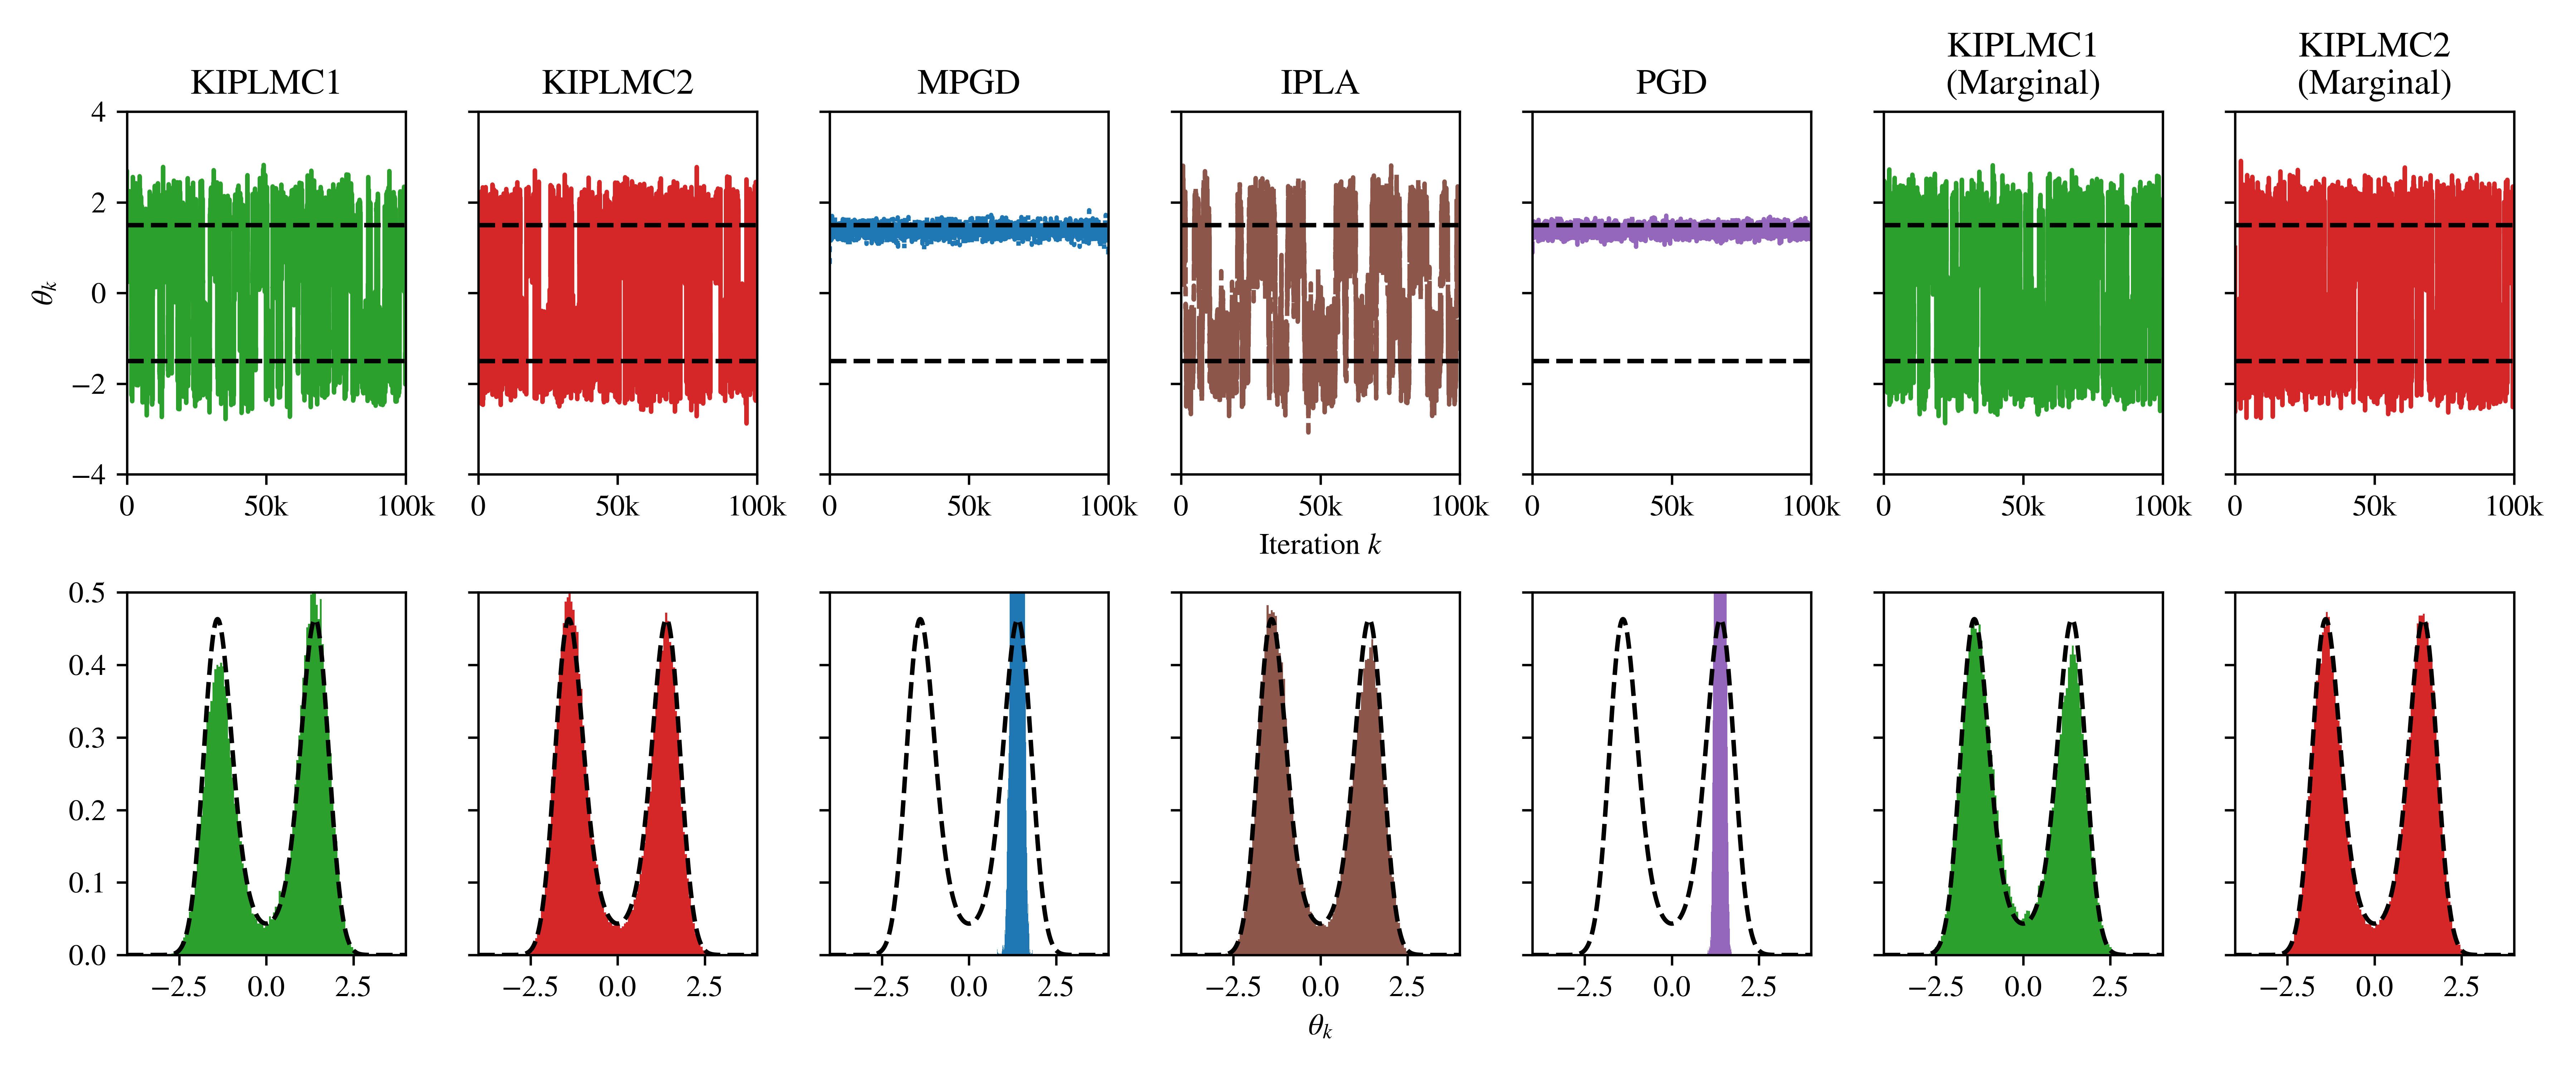
\includegraphics[width=\linewidth]{plots/fig5.png}
    \caption{\textbf{Multi-well Experiment.} The trace plots for \gls*{kiplmc1}, \gls*{kiplmc2}, \gls*{mpgd}, \gls*{ipla} and \gls*{pgd} on the multi-well experiment, together with density plots. The black dashed lines in the trace plots indicate the observationally equivalent data-generating parameter values $\theta=\pm1.5$, while the black dashed curves in the density plots show the target $\theta$-density proportional to $p_\theta(y)^N$. $N=10$, whilst the friction and step-size are optimised for each algorithm.}
    \label{fig:multiwell}
\end{figure*}
We include the following multi-well experiment to highlight the advantage of the noised $\theta$ dynamics, the core difference between the proposed methods and \gls*{mpgd} \citep{lim2023momentum}. To do this, we consider a synthetic example with a non-convex negative log-marginal-likelihood objective. Consider the joint probability density over $\mathbb{R}$,
\begin{align*}
    p_\theta(x,y) &= \mathcal{N}(y; x, \sigma^2_y)p_\theta(x),\\
    p_\theta(x) &= \frac{1}{2}\mathcal{N}(x; -\theta,\sigma^2_x) + \frac{1}{2}\mathcal{N}(x;\theta,\sigma_x^2).
\end{align*}
For $|y|>\sqrt{\sigma_x^2+\sigma_y^2}$, the marginal likelihood is bimodal as a function of $\theta$. Indeed, integrating out $x$ gives
\begin{equation*}
p_\theta(y) = \frac{1}{2} \mathcal{N}(y;\theta, \sigma_x^2+\sigma_y^2) + \frac{1}{2}\mathcal{N}(y;-\theta, \sigma_x^2 +\sigma_y^2).
\end{equation*}

In this case, we seek to show that whilst the \gls*{mpgd} algorithm gets stuck in one of the local minima, the \gls*{kiplmc1} algorithm escapes. For the experiment, we generate a single observation from the model with $\theta=1.5$, and we fix $\sigma_x^2=1$ and $\sigma_y^2=0.25$. Since $p_\theta=p_{-\theta}$, the values $\theta=\pm1.5$ are observationally equivalent data-generating parameter values; they need not coincide exactly with the maximisers of the marginal likelihood for the realised observation. In Fig.~\ref{fig:multiwell}, we show the trace plots of $\theta$ together with the associated empirical density plots, compared with these two reference values and the target $\theta$-density proportional to $p_\theta(y)^N$, respectively. For sake of comparison, we also compare the dynamics of \gls*{kiplmc1} and \gls*{kiplmc2} on the marginal dynamics, i.e. we consider \gls*{kipld} to be given simply as
\begin{align*}
\mathrm{d}\bm{\theta}_t &= \V_t^\theta \mathrm{d}t,\\
\mathrm{d}\V^\theta_t &= -\gamma \V_t^\theta\,\mathrm{d}t -\nabla_\theta \kappa(\bm{\theta}_t)\,\mathrm{d}t + \sqrt{\frac{2\gamma}{N}}\,\mathrm{d}\B_t,
\end{align*}
for an $\mathbb{R}^{d_\theta}$-valued Brownian motion $\B_t$. Recalling from Proposition~\ref{prop:stationary} that $\kappa(\theta)=-\log p_\theta(y)$, the invariant $\theta$-density of these marginal dynamics is proportional to $p_\theta(y)^N$. In Fig.~\ref{fig:multiwell}, all methods approach at least one of the two wells, but only the ``noised'' algorithms \gls*{kiplmc1}, \gls*{kiplmc2} and \gls*{ipla} reliably explore both wells.

\begin{figure}[t!]
    \centering
    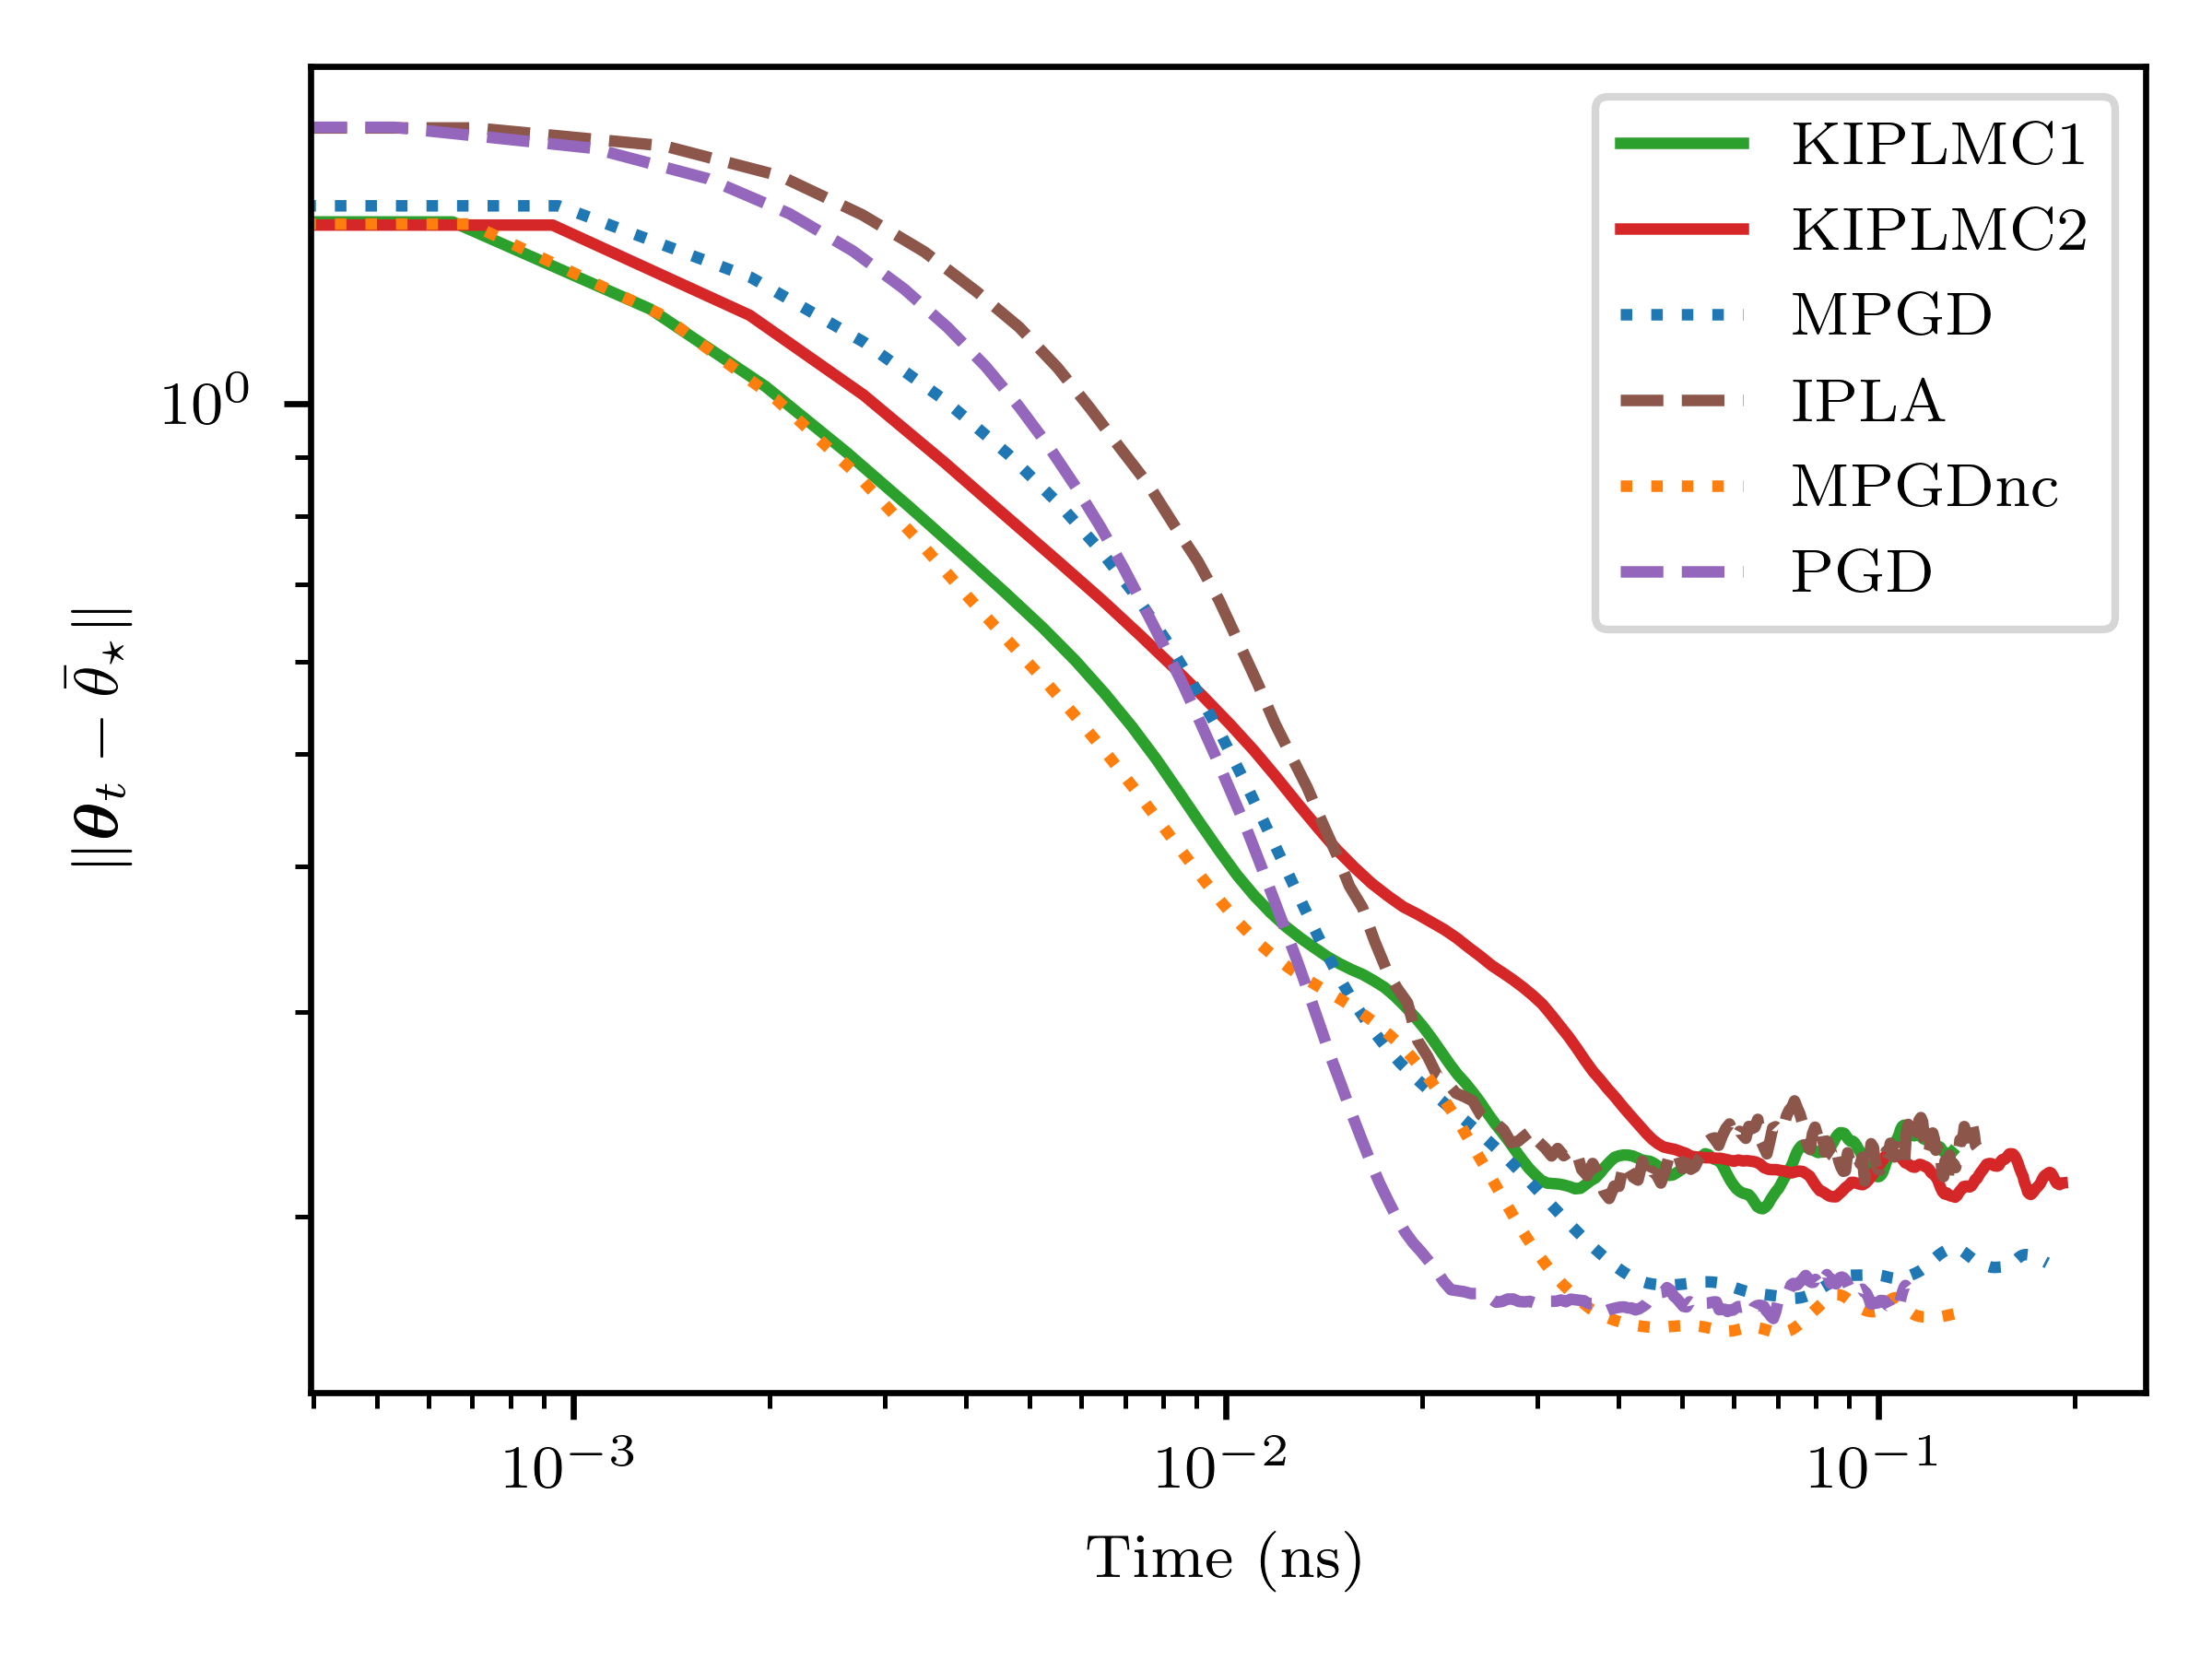
\includegraphics[width=.5\linewidth]{plots/timing.png}
    \caption{\textbf{Runtime Comparison.} We compare the MSE for the synthetic logistic regression experiment performed in Sec.~\ref{sec:toyex} with the same hyperparameters $d_x=d_\theta=3$, $d_y=100$, $\gamma=2.2$ and $N=100$. The results shown are the average of 100 Monte Carlo simulations.}
    \label{fig:timing}
\end{figure}

\subsection{Computational Cost Comparison}\label{app:compcost}
We further perform an additional experiment on the Sec.~\ref{sec:toyex} example, to compare MSE against computational cost. Indeed, this allows for more thorough comparisons with the methods, as \gls*{kiplmc1} generates correlated noise, \gls*{kiplmc2} performs a gradient correction and \gls*{mpgd} does both. Further all these methods require twice as much space in memory, when compared to \gls*{pgd} and \gls*{ipla}, due to the presence of the momentum variables.

In Fig.~\ref{fig:timing}, we observe the faster initial convergence rate of the momentum based methods, despite their greater computational cost. Further, we observe that the increased cost of noising the $\theta$-dynamics in our proposed methods, is negligible when compared to a second gradient evaluation per iteration, required by \gls*{mpgd} and \gls*{kiplmc2}.


\subsection{Area Between the Curves Calculation (ABC)}\label{sec:ABC}
To compare the behaviour of the different algorithms, we employ a measure that quantifies how accurately and quickly each algorithm converges to the true solution, namely the ABC, as in \citep{lim2023momentum}. Consider $c^k:\mathbb{N}\to \mathbb{R}$ and $c^m:\mathbb{N}\to \mathbb{R}$ to be the accuracy curves of \gls*{kiplmc2} and \gls*{ipla} respectively, i.e. for $\{\theta_n\}_{n=1}^\infty$ generated by the \gls*{kiplmc2} algorithm, $c^k(n)=\|\theta_n -\bar{\theta}^\star\|$. The ABC is given as,
\[\sum_{i=1}^M w(i) (c^m(i)-c^k(i)),\]
where $M$ is the total number of time-steps and $w$ acts as a weighting function $w(i)=2i/(M(M+1))$, matching \citep{kuntz2023particle}. Hence, the ABC computes a signed, weighted area between the error curves of \gls*{ipla} and \gls*{kiplmc2}. In particular, when $c^m$ is dominated by $c^k$, the ABC is negative, whilst positive in the converse case.


\subsection{Error Metrics for the BNN}\label{sec:err}
Recall that the output of our model for latent variable $x=(w,v)$, image features $f$ is,
\begin{equation*}
p(l|f, x) \propto \exp\left(\sum_{j=1}^{40} v_{lj} \tanh\left(\sum_{i=1}^{784} w_{ji} f_i\right)\right).
\end{equation*}
To normalise the outputs of the RHS over the labels we apply softmax to the estimates for all $l$. Denote this as $g(l|f,x)$ and we give the output of the model as
\begin{equation*}
\hat{l}(f|x) = \argmax_{l\in\{0,1\}} g(l|f,x).
\end{equation*}

For the BNN in \ref{sec:bnn} we use two metrics to evaluate the performance of our models, which we evaluate on test set of 200 images and labels $\mathcal{Y}_\text{test}$. In particular we use a relative error metric, measuring the percentage accuracy on the test set,
\begin{equation*}
\frac{1}{|\mathcal{Y}_\text{test}|}\sum_{(f,l)\in\mathcal{Y}_\text{test}} |l - \hat{l}(f|x)|.
\end{equation*}

Following \citep{kuntz2023particle}, our second metric is the log pointwise predictive density (LPPD),
\begin{equation*}
\frac{1}{|\mathcal{Y}_\text{test}|}\sum_{(f,l)\in\mathcal{Y}_\text{test}} \log g(l|f,x).
\end{equation*}
It is the average log probability assigned by the model to the correct test label; larger values indicate better predictive performance.
